In \cite{sb-umlfta} stellt sich heraus, dass der Abstand der separierenden Hyperebenen eines linearen Klassifikators $h_{(w,b)} \in \mathbb{H}$ zu den Datenvektoren ein geeignetes Gütemaß für die Generalisierungsfähigkeit für $h_{(w,b)}$ ist. Dieser Sachverhalt motiviert die Support-Vector-Machine (SVM): Die SVM liefert den linearen Klassifikator $h^*_{(w^*,b^*)}$, dessen Hyperebene $E_{(w^*,b^*)}$ den Abstand zu den Datenvektoren $(x^1,...,x^l)$ maximiert. Die SVM lässt sich damit als das Optimierungsproblem
\begin{equation}
	\label{equ-svm-1}
	\begin{aligned}
	\argmax_{||w||=1} { \; \min_{1 \leq i \leq l}{ \; d(E_{(w,b)}, x^i) }} \qquad
					  \text{u.d.N.} \qquad h_{(w,b)} \in \mathbb{H}
 	\end{aligned}
\end{equation}
auffassen. In anderer Notation aufgeschrieben (siehe Lemma \ref{lemma-abstand-norm}, Definition \ref{def-lin-sep}, sowie Gleichung (\ref{equ-H})) ergibt dies
\begin{equation}
	\label{svm-min-max-nb}
	\begin{aligned}
		& \smash{ \argmax_{\substack{||w||=1 \\ (w,b) \in \mathbb{R}^n \times \mathbb{R}}}{ 
			\min_{1\leq i \leq l}{y^i(\langle w, x^i \rangle + b)}
		}} \qquad \text{u.d.N.} \qquad &
		y^i(\langle w, x^i \rangle + b) > 0 \\ 
		&& i = 1,...,l
	\end{aligned}
\end{equation}
Wir wollen nun zeigen, dass (\ref{equ-svm-1}) eine Lösung besitzt. Dies ist nicht unmittelbar klar, da $\mathbb{H}$, wie in Satz \ref{satz-svm-ls} zu sehen ist, nicht abgeschlossen ist (wenn man als Norm den Abstand der korrespondieren Ebenen heranzieht). Um die Lösbarkeit zu zeigen, werden wir (\ref{svm-min-max-nb}) geeignet umformulieren. Zunächst zeigen wir die Äquivalenz von (\ref{svm-min-max}) mit

\begin{equation}
\label{svm-min-max}
\begin{aligned}
	\argmax_{\substack{||w||=1 \\ (w,b) \in \mathbb{R}^n \times \mathbb{R}}}{
		\min_{1\leq i \leq l}{y^i(\langle w, x^i \rangle + b)}
	}.
\end{aligned}
\end{equation}

Anschließend führen wir die \emph{Hard-SVM} (Definition \ref{hard-svm}) ein. In Lemma \ref{lemma-svm-prob-aequ} ergibt sich schließlich die Äquivalenz aller drei Probleme. In Lemma \ref{lemma-hard-svm-loes} wird abschließend die Lösbarkeit von (\ref{hard-svm}) und damit die Lösbarkeit von (\ref{equ-svm-1}) gezeigt.

\begin{lemma}
	\label{lemma-svm-minmax-equ}
	Angenommen die Probleme (\ref{svm-min-max}) und (\ref{svm-min-max-nb}) sind lösbar. Dann sind beide Probleme äquivalent.
\end{lemma}
\begin{proof}
	Sei $(w^*,b^*)$ eine Lösung von (\ref{svm-min-max-nb}) und $(\bar{w},\bar{b})$ eine Lösung von (\ref{svm-min-max}).
	Dann ist wegen der Separierbarkeit der Trainingsdaten $\min_{1\leq i \leq l}{y^i\langle \bar{w}, x^i \rangle + \bar{b}} > 0$. Also ist $(\bar{w},\bar{b})$ zulässig für \ref{svm-min-max-nb}. Damit ist $y^i\langle \bar{w}, x^i \rangle + \bar{b} \leq y^i\langle w^*, x^i \rangle + b^*$. Da offensichtlich $(w^*,b^*)$ zulässig für \ref{svm-min-max} ist, gilt schon $y^i\langle \bar{w}, x^i \rangle + \bar{b} = y^i\langle w^*, x^i \rangle + b^*$. Damit ist die Behauptung gezeigt.
\end{proof}

Wir definieren nun die eingangs erwähnte Hard-SVM. Sie zeichnet sich durch die Abeschlossenheit ihrer Nebenbedingungen aus.
\begin{definition}[Hard-SVM]
	Das durch
	\begin{equation}
	\label{hard-svm}
	\begin{aligned}
		& \smash{\argmin_{(w,b) \in \mathbb{R}^n \times \mathbb{R}}{ \; \frac{1}{2}||w||^2}} \qquad
		\text{u.d.N.} \qquad & 
		y^i(\langle w, x^i \rangle + b) \geq 1 \\
		&& i = 1,...,l
	\end{aligned}
	\end{equation}
	definierte Optimierungproblem bezeichnen wir als Hard-SVM.
\end{definition}

\begin{lemma}
	\label{lemma-hard-svm-loes}
	Das quadratische Optimierungsproblem (\ref{hard-svm}) besitzt eine Lösung.
\end{lemma}
\begin{proof}
Seien $(\tilde{w}, \tilde{b})$ zulässig für (\ref{hard-svm}). Wegen der Separierbarkeit  existieren solche $(\tilde{w},\tilde{b})$. Um die Lösbarkeit von (\ref{hard-svm}) zu zeigen, dürfen wir die Suche nach einem Minimum auf das Gebiet 
$G = \{ (w, b) \in \mathbb{R}^n \times \mathbb{R} \mid ||w|| \leq || \tilde{w}|| \}$ 
beschränken. 
Analog zum Satz \ref{satz-svm-ls} kann gezeigt werden, dass mit
$$
	M' := \max_{||w|| \leq || \tilde{w}||}{\max_{1 \leq i \leq l}{y^i \langle w, x^i \rangle}}.
$$
(vgl. (\ref{equ:bounded-set})) die Bedingung $|b| < M'$ für ein beliebiges $(w,b) \in G$ gelten muss, sodass sich Gebiet weiter auf  $\{ (w, b) \in \mathbb{R}^n \times \mathbb{R} \mid ||w|| \leq ||\tilde{w}||, |b| \leq M \}$ einschränken lässt. Vorliegend haben wir also eine stetige Zielfunktion mit einer abgeschlossenen und beschränkten - nach dem Satz von Heine-Borel (\cite{ae-ana1}) also kompakten - Menge als zulässigen Bereich. Nach dem Satz vom Mimimum und Maximum (\cite{ae-ana1}) ist das Problem (\ref{hard-svm}) also lösbar.
\end{proof}

\begin{bemerkung}
\label{bem-hard-svm}
\begin{itemize}
\item[(a)] Es wird noch ersichtlich, dass die Ungleichungen in den Nebenbedingungen für gewisse $i \in \{1,...,l\}$ aktiv sind. Man nennt die Vektoren $x^i$ für solche $i \in \{1,...,l\}$ auch Support-Vektoren. Weiter werden wir sehen, dass die Lösung im Wesentlichen bereits durch die Support-Vektoren bestimmt ist. Genauer gilt für eine Lösung $(w^*,b^*)$ von (\ref{hard-svm}) die Beziehung 
$$
w^* = \sum_{i=1}^{l} \alpha_i x^i,
$$ 
für gewisse nicht negative $\alpha_1,...,\alpha_l \in \mathbb{R}^+_0$. 
\item[(b)] Sei $w^*$ eine Lösung für (\ref{hard-svm}) und $x^i$ ein Support-Vektor. Aus (a) folgt, dass $$
y^i(\langle w^*, x^i \rangle + b) = 1 
\Leftrightarrow 
\frac{y^i}{||w^*||}(\langle w^*, x^i \rangle + b) = \frac{1}{||w^*||} \Leftrightarrow
d(E_{(w,b)},x^i) = \frac{1}{||w^*||}
$$
gilt. Nach Lemma \ref{lemma-abst-hyp-allg} minimiert (\ref{hard-svm}) also den Abstand der Hyperebene $(w,b)$ zu den Datenvektoren. Intuitiv ergibt sich, dass die Probleme (\ref{hard-svm}), (\ref{svm-min-max-nb}), (\ref{svm-min-max}) äquivalent sind.
\item[(c)] Den Abstand einer Hyperebene zu den Datenvektoren nennt man auch Margin.
\end{itemize}
\end{bemerkung}

\begin{figure}
	\centering
	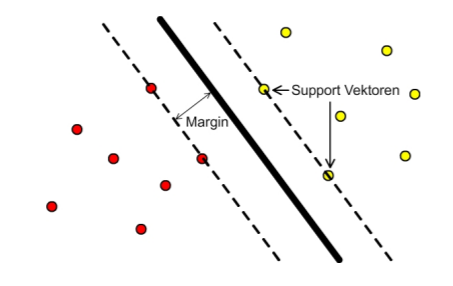
\includegraphics{abbildungen/sv.PNG}
	\caption{Die Abbildung zeigt die optimale trennende Hyperebene zwischen den gelben und roten Datenvektoren, sowie die jeweiligen Support-Vektoren.}
	\label{img:sv}
\end{figure}

Wir wollen abschließend die Überlegung aus \ref{bem-hard-svm} (b), sowie die Lösbarkeit und Äquivalenz der Probleme (\ref{svm-min-max-nb}), (\ref{svm-min-max}) und (\ref{hard-svm}) in einem Lemma festhalten.

\begin{lemma}
	\label{lemma-svm-prob-aequ}
	Die Probleme (\ref{svm-min-max-nb}), (\ref{svm-min-max}) sowie (\ref{hard-svm}) sind äquivalent und lösbar.
\end{lemma}
\begin{proof}
	Die Äquivalenz von den Problemen (\ref{svm-min-max}) und (\ref{hard-svm}) folgt (nach einer Normierung der Zielfunktion um den Faktor $2$) mit Lemma 15.2 in \cite{sb-umlfta}. Die Aussage folgt dann mit Lemma \ref{lemma-svm-minmax-equ} und Lemma \ref{lemma-hard-svm-loes}.
\end{proof}

\section{Homogene SVMs}
Die \emph{homogene SVM} überführt zunächst die separierbaren Datenvektoren $(x^1,y^1),...,(x^l,y^l)$ über die \emph{Einbettung}
$$
\widehat{(\, \cdot \, )} : \mathbb{R}^n \rightarrow \mathbb{R}^{n+1},\ \hat{x} := (x,1).
$$
in den $\mathbb{R}^{n+1}$. Die eingebetteten Datenvektoren kennzeichnen wir mit
$$
\hat{x}^1,...,\hat{x}^l \in \mathbb{R}^n \times \mathbb{R} = \mathbb{R}^{n+1}.
$$
Es ist ersichtlich, dass die eingebetteten Datenvektoren $\hat{x}^1,...,\hat{x}^l$ durch eine homogene Hyperebene $E_{(\tilde{w},0)} \subset \mathbb{R}^{n+1}$ separiert werden können. Analog zum Hard-SVM wählt die homogene SVM nun die homogene Ebene, die den Abstand zu den eingebetteten Datenvektoren maximiert. Dies führt uns wie im vorherigen Unterkapitel auf die

\begin{definition}[Homogene SVM]
Das durch 
\begin{equation}
\label{equ-homog-svm}
\begin{aligned}
	\min_{\tilde{w} \in \mathbb{R}^{n+1}} \; \frac{1}{2} ||\tilde{w}||^2 \qquad
	\text{u.d.N.} \qquad  
	y^i \langle \hat{x}^i, \tilde{w} \rangle \geq 1
\end{aligned}
\end{equation}
definierte Optimierungsproblem bezeichnen wir als homgene SVM.
\end{definition}

\begin{bemerkung}
\begin{itemize}
\item[(a)] Die Lösbarkeit von (\ref{equ-homog-svm}) kann analog zum Lemma \ref{lemma-hard-svm-loes} gezeigt werden. 
Fassen wir $\tilde{w}$ als $(w,b) \in \mathbb{R}^n \times \mathbb{R}$ auf, lässt sich die homogene SVM auch in der Form
$$
\begin{aligned}
\min_{(w,b)} \; \frac{1}{2} \left( ||w||^2 + b^2 \right) \qquad
\text{u.d.N.} \qquad  y^i (\langle x^i, w \rangle +b) \geq 1
\end{aligned}
$$
schreiben. Damit kann die homogene SVM als Hard-SVM aufgefasst werden, bei der zusätzlich der Term $b$ regularisiert wird.
\item[(b)] Wir werden im nächsten Unterkapitel sehen, dass bei der Dualisierung der homogenen SVM eine Nebenbedingung wegfällt. Dies wird uns später bei der Formulierung der Koordinatenabstiegsmethode sehr zu pass kommen.
\item[(c)] Das Beispiel \ref{bsp-homg-nequ-hard} zeigt, dass sich die Lösungen der Hard-SVM und der homogenen SVM im Allgemeinen unterscheiden. Nach \cite{sb-umlfta} ist dieser Unterschied für das Klassifizierungsproblem in der Praxis jedoch oft nicht spürbar.
\end{itemize}
\end{bemerkung}
 
\begin{beispiel}
\label{bsp-homg-nequ-hard}
Seien
$$
\begin{aligned}
	x^1 &= (1,\ 2)^t  &x^2  &= (1,\ 0)^t \\
	y^1 &= 1 		  &y^2 &= -1
\end{aligned}
$$
die Datenvektoren für die beiden Klassen $L=\{ y^1,\ y^2 \} = \{1,\ -1 \}$. Nach einer Modifikation für das homogene SVM erhalten wir 
die Datenvektoren
$$
\begin{aligned}
	\hat{x}^1 &= (1,\ 2,\ 1)^t &\hat{x}^2 &= (1,\ 0,\ 1)^t \\
	 y^1 &= 1					 &y^2 &= -1
\end{aligned}.
$$


\begin{figure}[htbp]
	\centering
	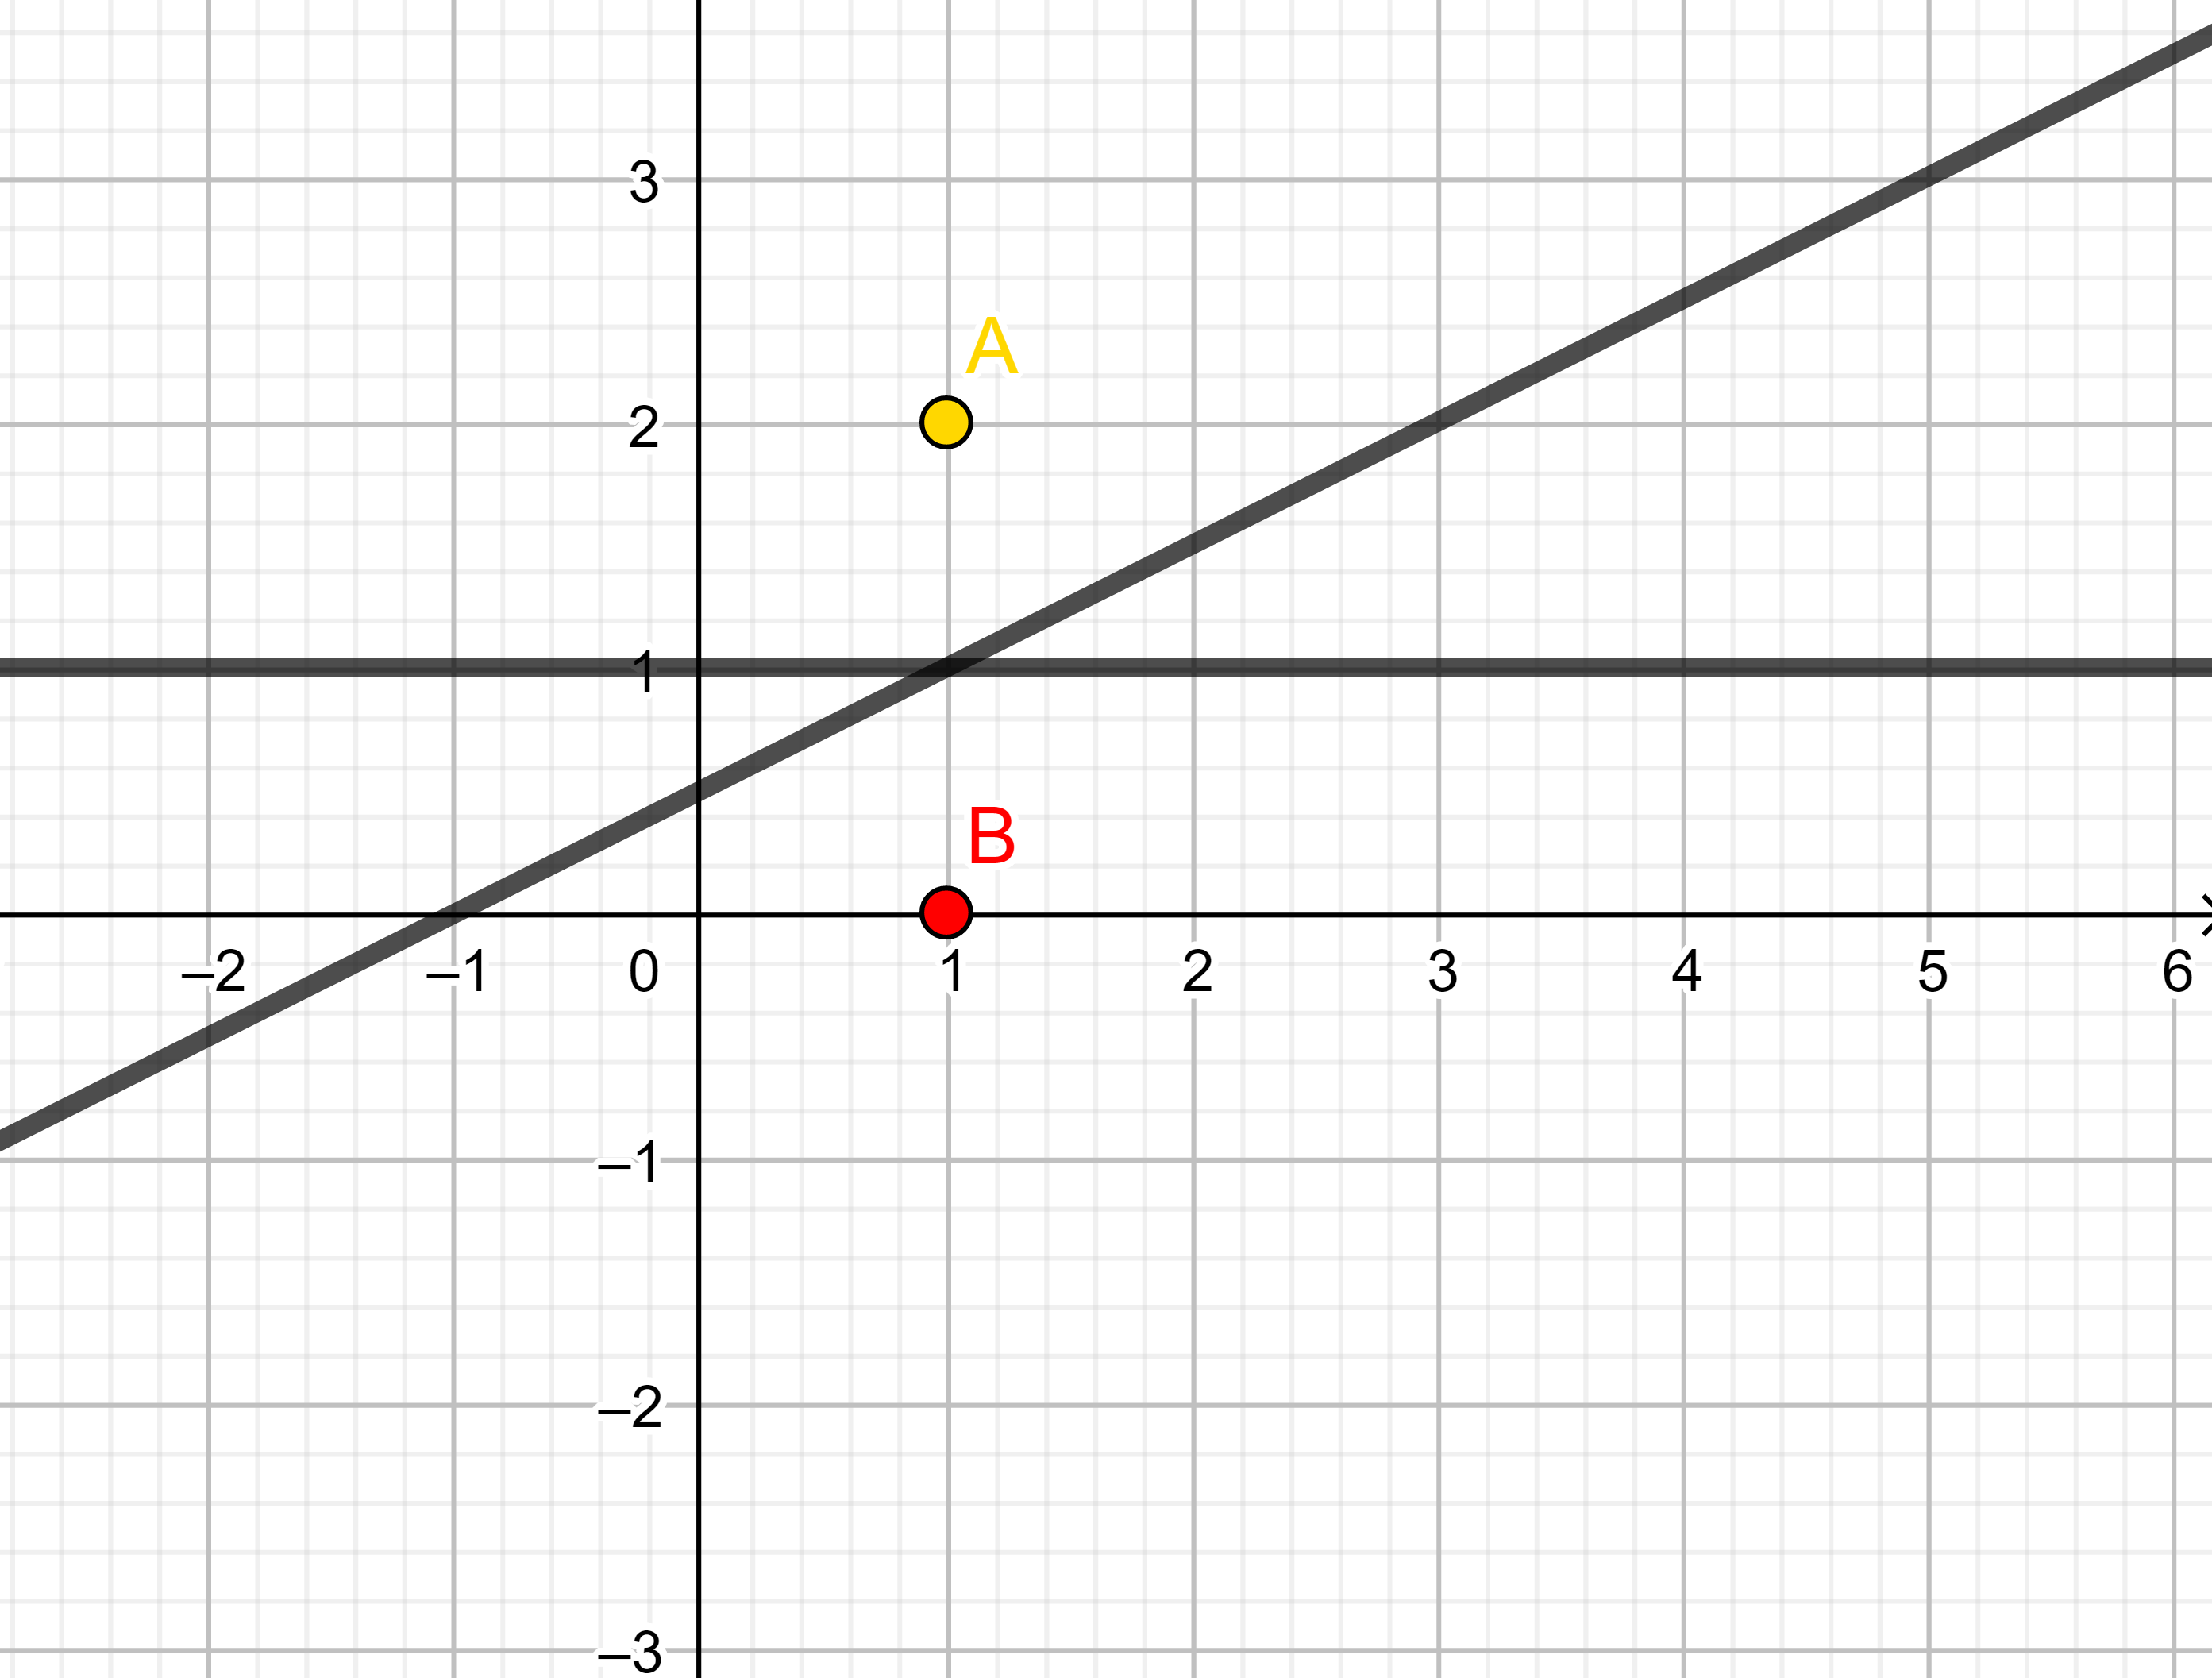
\includegraphics{abbildungen/homogen.png}
	\caption{Die Abbildung zeigt die Lösung vom Hard- bzw. homogenen SVM für die Datenvektoren $A=x^1 = (1, 2)^t$ und $B=x^2 = (1,0)^t$ im $\mathbb{R}^2$.}
	\label{img:hardvssoft}
\end{figure}

Für das Hard- bzw. homogene SVM ist eine Hyperebene $(w,b) \in \mathbb{R}^{2+1}$ bzw. $\tilde{w} := (w,b) \in \mathbb{R}^{3}$ gesucht, die den Restriktionen
$$
\begin{aligned}
	w_1 + 2w_2 + \, b -1 \geq 0 \\
	w_1 + \, b +1 \geq 0,
\end{aligned}
$$
beziehungsweise 
$$
\begin{aligned}
	0 &\geq -w_1 - 2w_2 - b + 1 \\
	0 &\geq  w_1 + b + 1
\end{aligned}
$$
genügt, wobei $w_i$ die i-te Komponente von $w$ bezeichnet. Während die Restriktionen bei der Hard- und homogenen SVM übereinstimmen, ändert sich bei der homogenen SVM die Zielfunktion von
$$
	\min_{(w,b)} \; \frac{1}{2} (w_1^2+w_2^2).
$$
zu
$$
	\min_{(w,b)} \; \frac{1}{2} (w_1^2+w_2^2+b^2).
$$
Wie auf der Abbildung \ref{img:hardvssoft} zu erkennen ist, ergibt sich die normierte Lösung der Hard-SVM durch die Hyperebene $\{ (x_1,x_2) \in \mathbb{R}^2 \ | \ x_2=1 \} \subset \mathbb{R}^2$. 
Um die Lösung der homogenen SVM zu ermitteln, suchen können wir das Gleichungssystem
$$
	\nabla \left( \frac{1}{2}(w_1^2+w_2^2+b^2) \right) = 
	\begin{pmatrix} w_1 \\ w_2 \\ b \end{pmatrix} = 
	\begin{pmatrix} 
		-\lambda_1 + \lambda_2 \\ -2 \lambda_1 \\ -\lambda_1 + \lambda_2 
	\end{pmatrix} = 
	- \lambda_1 \begin{pmatrix} 1 \\ 2 \\ 1 \end{pmatrix} +
	\lambda_2 \begin{pmatrix} 1 \\ 0 \\ 1 \end{pmatrix}
$$
lösen. Erhalten wir damit einen KKT-Punkt, müssen wir diesen Schritt nicht näher erläutern. Eingesetzt in die Restriktionen ergibt dies
$$
\begin{aligned}
	6 \lambda_1 & - 2 \lambda_2 \geq 1 \\
	-2 \lambda_1 &+ 2 \lambda_2 \geq 1,
\end{aligned}
$$
woraus $\lambda_1 \geq \frac{1}{2} ,\ \lambda_2 \geq 1$ folgt. Um einen KKT-Punkt zu erhalten setzen wir schließlich $\lambda_1 = \frac{1}{2} ,\ \lambda_2=1$. Damit ist $(w_1, w_2, b) = (\tfrac{1}{2}, -1, \tfrac{1}{2})$. Die Hyperebene im $\mathbb{R}^2$ ist also durch $ \{ (x_1,x_2) \in \mathbb{R}^2 \ | \ \tfrac{1}{2}x_1-x_2+\tfrac{1}{2} = 0  \} \subset \mathbb{R}^2$ gegeben.
\end{beispiel}


Um die Notationen zu vereinfachen werden wir im homogenen Fall immer annehmen, dass die Trainingsdaten a priori in den $\mathbb{R}^{n+1}$ eingebettet wurden. Wir können in diesem Fall also wieder davon ausgehen, dass $\hat{x}^i \in \mathbb{R}^n$ und schreiben $x^i$ statt $\hat{x}^i$, sowie $w$ statt $\tilde{w}$. Auch in den nächsten Abschnitten werden wir dies so fortführen.

\section{Soft-SVMs}
Wir wollen zunächst anmerken, dass wir für die \emph{Soft-SVM} wieder den homogenen Fall annehmen. \\

Die lineare Separierbarkeit (Definition \ref{def-lin-sep}) ist eine sehr harte Anforderung an die Datenvektoren $(x^1,y^1),...,(x^l,y^l)$ und in der Praxis nicht immer anzutreffen. Aus diesem Grund führen wir in der nächsten Definition ein neues Problem ein, das die Anforderung durch die \emph{Schlupfvariable} $\xi = (\xi_1 ,...,\xi_l) \in \mathbb{R}^l$ abschwächt.

\begin{figure}[h]
	\centering
	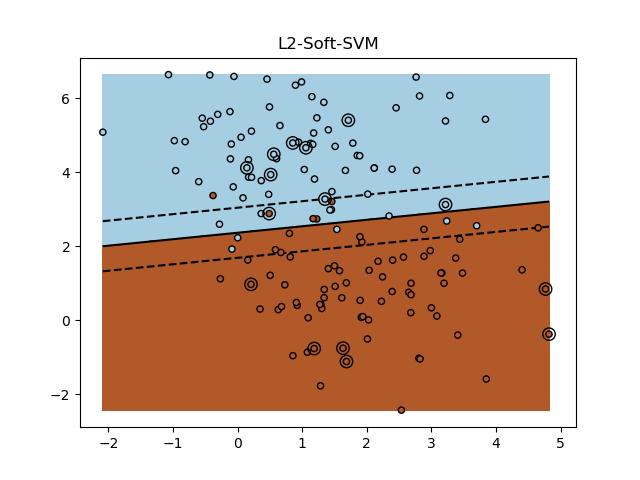
\includegraphics[scale=0.90]{abbildungen/softsvm_ex1.png}
	\caption{Illustrierung eines Klassifizierungsproblems. Die schwarze durchgezogene Linie zeigt die durch die L2-Soft-SVM ermittelte Hyperebene. Die gestrichelte Linie deutet den Margin an. (Die doppelt umrandeten Datenvektoren haben nicht zur Modellbildung beigetragen. Bei diesen Vektoren handelt es sich also um \emph{Testvektoren}.)}
	\label{img:softsvm}
\end{figure}

\begin{definition}[L1/L2-Soft-SVM]
	Seien $p=1,2,\ C > 0$. Dann ist die Lp-Soft-SVM definiert durch
	\begin{equation}
	\label{soft-svm-slack1}
	\begin{aligned}
		& \smash{ \argmin_{(w,\xi) \in \mathbb{R}^n \times \mathbb{R}^l}{
			\frac{1}{2}||w||^2+C\sum_{i=1}^{l}{\xi_i^p}
		}}
		\qquad \text{u.d.N.} \qquad
		& y^k \langle w, x^k \rangle &\geq 1 - \xi_k \\
		&& \xi_k &\geq 0 \\
		&& k &= 1,...,l.
	\end{aligned}
	\end{equation}
\end{definition}
Zu erkennen ist, dass der Schlupf $\xi$ die Lösbarkeit von $(\ref{soft-svm-slack1})$ sicherstellt; auch dann, wenn die Datenvektoren $(x^1,y^l),...,(x^l,y^l)$ nicht separierbar sind.

Definieren wir $$\ell_i^p(x,b) := \max(1-y^i\langle w, x^i \rangle,\ 0)^p,$$ für $i=1,...,l$, so stoßen wir auf die
\begin{definition}[SVM mit L1/L2 hinge loss]
	Seien $p=1,2,\ C > 0$. Dann ist die $L_p$-Soft-SVM mit \emph{hinge-loss} definiert durch
	\begin{equation}
	\label{soft-svm-loss1}
	\begin{aligned}
	\argmin_{w \in \mathbb{R}^n}{\frac{1}{2}||w||^2+C\sum_{1}^{l}{\ell_i^p(w)}}.
	\end{aligned}
	\end{equation}
\end{definition}

\begin{lemma}
	\label{lemma-soft-loesbar}
	Die Probleme (\ref{soft-svm-slack1}) und (\ref{soft-svm-loss1}) sind lösbar und äquivalent. 
\end{lemma}
\begin{proof}
	Ein Beweis wird in Behauptung 15.5 \cite{sb-umlfta} für den Fall $p=1$ geliefert: Fixiere $(w,b)$ und minimiere über $\xi$ bezüglich des Problems (\ref{soft-svm-slack1}). Wegen $\xi \geq 0$ ist $\xi_i = 0$, genau dann wenn $y^i(\langle w, x^i \rangle +b) \geq 1$ und $\xi_i = 1-y^i(\langle w, x^i \rangle +b)$ im anderen Fall. Da $(w,b)$ beliebig waren, gilt dies auch für das Minimum. Damit ist die Behauptung gezeigt. Den Fall $p=2$ zeigt man analog.
\end{proof}

\section{Duale SVM-Probleme}
Im Folgenden werden wir die \emph{dualen Probleme} der vorherigen \emph{primalen Probleme} herausarbeiten. Sie sind oft - auch in dieser Arbeit - Grundlage algorithmischer Lösungsverfahren. Zunächst zeigen wir jedoch ein vorbereitendes Hilfslemma.

\begin{lemma}
	Seien $\alpha \geq 0 \in \mathbb{R}^n$,
	\begin{equation}
	\begin{aligned}
	G_{\alpha}: \mathbb{R}^n \rightarrow \mathbb{R}, w \mapsto \frac{1}{2}||w||^2 + \sum_{i=1}^{l} \alpha_i (1- y^i( \langle w, x^i \rangle)), \\
	q(\alpha) := \sum_{i=1}^{l}\alpha_i - \frac{1}{2} \left< \sum_{j=1}^{l} \alpha_j y^j x^j ,\ \sum_{j=1}^{l} \alpha_j y^j x^j \right>.
	\end{aligned}
	\end{equation}Die Funktion $G_\alpha$ besitzt ihr Minimum bei $w^* = \sum_{1}^{l} \alpha_i y^i x^i$. Weiter ist $G_{\alpha}(w^*) = q(\alpha)$.
\end{lemma}
\begin{proof}
	Nach Satz \ref{satz-strict-konvex-innprdt} ist der erste Summand von $G_\alpha$ konvex. Da der zweite Summand als lineare Funktion konvex ist und Linearkombinationen konvexer Funktionen konvex sind, ist $G_\alpha$ konvex. Nach Satz \ref{dual-kkt} ist $G_{\alpha}(w)$  also genau dann minimal, wenn $(w)$ ein KKT-Punkt ist. Aus der ersten KKT-Bedingungen ergibt sich für das Minimum von $G_\alpha$ die Bedingung $\nabla G_\alpha(w) = w - \sum_{i=1}^{l} \alpha_i y^i x^i = 0 \Leftrightarrow w = \sum_{i=1}^{l} \alpha_i y^i x^i$. Die letzte Behauptung zeigt die Rechnung 
	$$
	\begin{aligned}
	G_\alpha(w^*) &= \left | \left |\sum_{1}^{l} \alpha_i y^i x^i \right | \right |^2 +
	\sum_{i=1}^l \alpha_i \left (1-y^i \left \langle \sum_{1}^{l} \alpha_i y^i x^i, x^i \right \rangle \right ) = \\
	&=\sum_{i=1}^{l}\alpha_i - \frac{1}{2} \left< \sum_{j=1}^{l} \alpha_j y^j x^j ,\ \sum_{j=1}^{l} \alpha_j y^j x^j \right> = q(\alpha).
	\end{aligned}
	$$
\end{proof}

Für den nächsten Satz merken wir noch an, dass die primalen Probleme aus konvexen und stetig differenzierbaren Zielfunktionen sowie affin linearen Nebenbedingungen bestehen, sodass die im Anhang vorgestellte Dualitätstheorie für restringierte Optimierungsprobleme in ihrer Gänze anwendbar ist.

\begin{satz}[Die dualen SVM-Probleme]
	\label{satz-svm-dual-probleme}
	Sein $q$ und $G_\alpha$ wie im vorherigen Lemma definiert. Es gelten die Aussagen:
\begin{itemize}
	\item[(i)] Das duale Problem der Hard-SVM lautet $\max_{\alpha \geq 0} q(\alpha)$ u.d.N. $\sum_{i=1}^l \alpha_i y^i = 0$.
	\item[(ii)] Das duale Problem der homogenen SVM lautet $\max_{\alpha \geq 0} q(\alpha)$.
	\item[(iii)] Das duale Problem der L1-Soft-SVM lautet $\max_{C \geq \alpha \geq 0} q(\alpha)$
	\item[(iv)] Das duale Problem der L2-Soft-SVM mit lautet $\max_{\alpha \geq 0} q(\alpha)-\frac{1}{4C}\sum_{i=1}^{l} \alpha_i^2$.
\end{itemize}
\end{satz}
\begin{proof}
Zu (i): Die \emph{Lagrange-Funktion} für die Hard-SVM ist
$$
L(w,b,\alpha) = \frac{1}{2}||w||^2 + \sum_{i=1}^{l}\alpha_i(1-y^i(
\langle w,x^i \rangle) + b) = G_{\alpha}(w) - \sum_{i=1}^{l}\alpha_i y^i b.
$$
Für $\sum_{i=1}^{l}y^i \alpha_i \neq 0$ ist $\inf_{(w,b)} L(w,b,\alpha) = -\infty$, weshalb wir uns für das duale Problem auf $\sum_{i=1}^{l}y^i \alpha_i = 0$ beschränken können. Das duale Problem der Hard-SVM ist damit gegeben durch
$$
\begin{aligned}
\max_{\alpha \geq 0} \inf_{(w,b)} L(w,b,\alpha) = 
\max_{\alpha \geq 0} \min_w G_{\alpha}(w) = \max_{\alpha \geq 0}q(\alpha) \\
\text{u.d.N} \; \sum_{i=1}^l \alpha_i y^i = 0.
\end{aligned}
$$.

Zu (ii): Die Lagrange-Funktion für die homogene SVM ist
$$
L(w,\alpha) = \frac{1}{2}||w||^2 + \sum_{i=1}^{l}\alpha_i(1-y^i 
\langle w,x^i \rangle) = G_{\alpha}(w).
$$
Das duale Problem der homogenen SVM ist damit gegeben durch
$$
\max_{\alpha \geq 0} \inf_{(w,b)} L(w,b,\alpha) = 
\max_{\alpha \geq 0} \min_w G_{\alpha}(w) = \max_{\alpha \geq 0}q(\alpha)
$$.


Zu (iii): Die Lagrange-Funktion vom Problem \ref{soft-svm-slack1} ist gegeben durch 
$$
\label{lagrange-l1-softsvm1}
\begin{aligned}
L(w, \xi, \alpha, \beta) &:= \tfrac{1}{2}||w||^2 + C \sum_{i=1}^l \xi_i 
+ \sum_{i=1}^{l}{\alpha_i (1-y^i w^t x^i - \xi_i)} - \sum_{i=1}^{l} \beta_i \xi_i = \\
&= \tfrac{1}{2} ||w||^2 + \sum_{i=1}^{l}{\alpha_i (1-y^i w^t x^i)} + \sum_{i=1}^{l}(C-\alpha_i - \beta_i)\xi_i \\
&= G_{\alpha}(w) + \sum_{i=1}^{l}(C-\alpha_i - \beta_i)\xi_i.
\end{aligned}
$$
Für $C \neq \alpha_i + \beta_i$ für ein $i \in \{1, ..., l\}$ ist $\inf_{w,\xi}L(w,\xi,\alpha,\beta) = -\infty$. Wir dürfen also für das duale Problem $C_i = \alpha_i+\beta_i$ für alle $i = 1,...,l$ annehmen. Also muss die Bedingung $0 \leq \alpha \leq C$ gelten. Das duale Problem der L1-Soft-SVM ist damit gegeben durch
$$
\max_{C \geq \alpha \geq 0} \inf_{(w,b)} L(w,b,\alpha) = 
\max_{C \geq \alpha \geq 0} \min_w G_{\alpha}(w) = \max_{C \geq \alpha \geq 0}q(\alpha).
$$

Zu (iv): Die Lagrange-Funktion ist damit gegeben durch
$$
\begin{aligned}
L(w,\xi,\alpha,\beta) &= \frac{1}{2}||w||^2+\sum_{i=1}^l \alpha_i(1-y^i \langle w, x^i \rangle ) + \sum_{i= 1}^l \left(C \xi_i^2 - \alpha_i \xi_i - \beta_i \xi_i \right) \\
&= G_\alpha(w) + \sum_{i= 1}^l \left(C \xi_i^2 - \alpha_i \xi_i - \beta_i \xi_i \right).
\end{aligned}
$$
Der von $\xi$ abhängige Term ist nach Satz \ref{dual-kkt} minimal bei $\xi = \tfrac{1}{2}(\alpha + \beta)$. Nach Satz \ref{dual-satz} ist die duale Lösung gepaart mit einer primalen Lösung ein KKT-Punkt. Für eine mögliche Lösung muss also wegen des Komplementären Schlupfs $\beta^t \xi = 0$ gelten. Wegen $\beta \geq 0, \alpha \geq 0$ erhalten wir insgesamt, dass für eine duale Lösung $\beta  = 0$ gelten muss. Das duale Problem der L2-Soft-SVM ist damit gegeben durch
$$
\begin{aligned}
\max_{\alpha \geq 0, \beta \geq 0} \inf_{w,\xi \geq 0} L(w,\xi,\alpha,\beta) =
\max_{\alpha \geq 0} 
q(\alpha) + \sum_{i= 1}^l C(\tfrac{1}{2C}\alpha)^2 - \tfrac{1}{2C} \alpha^2 = 
\max_{\alpha \geq 0} q(\alpha) - \sum_{i= 1}^l \tfrac{1}{4C}a_i^2.
\end{aligned}
$$
\end{proof}

\begin{bemerkung}\label{bem:duale-probleme}
\begin{itemize}
\item[(a)] Die Lösbarkeit der dualen Probleme aus dem vorherigen Satz sieht man mit Hilfe von Satz \ref{dual-kkt}, Satz \ref{dual-satz} und der bereits gezeigten Lösbarkeit der jeweiligen primalen Probleme.
\item[(b)]
Für den Fall (i) aus dem vorherigen Satz zeigen wir exemplarisch, wie wir aus der dualen Lösung $\alpha^*$ die primale Lösung $(w^*,b^*)$ erhalten. Wegen  Satz \ref{dual-satz} ist $(w^*,b^*,\alpha^*)$ ein KKT-Punkt. Aus den KKT-Bedingungen folgt, dass 
$$
\nabla_w L(w^*,b^*,\alpha^*) = 0 \Leftrightarrow \nabla G_{\alpha^*}(w^*) = 0 \Leftrightarrow w^* = \sum_{i=1}^{l}y^i \alpha_i^* x^i.
$$ 
Um $b^*$ zu ermitteln, sei hierzu ein $i \in \{1, ..., l\}$ mit $\alpha_i^* > 0$. Wegen des komplementären Schlupfs gilt dann 
$$
1-y^i(\langle w^*, x^i \rangle) + b^* = 0 \Leftrightarrow b^* = -1+y^i(\langle w^*, x^i \rangle).
$$
\item[(c)]
\label{svm-eindeutigkeit}
Für die Fälle (ii) bis (iv) gilt mit analoger Begründung die Beziehung 
$w^* = \sum_{i=1}^{l}y^i \alpha_i^* x^i$ wobei $w^*$ und $\alpha^*$ die jeweiligen Teillösungen der primalen bzw. dualen Probleme sind. 
Weiter folgt aus den Fällen (iii) und (iv), dass mit $\xi^* = \ell^1(w^*):=(\ell_1^1(w^*),...,\ell_l^1(w^*))$ der Vektor $(w^*,\xi^*)$ eine Lösung für das jeweilige primale Problem ist.

\item [(d)] Aus (b) und (c) folgen, dass die primale Lösung für die Probleme (i) bis (iv) eindeutig bestimmt sind.

\item[(e)] Führt man für die Hard-SVM analog zur Soft-SVM Schlupfvariablen ein, ist die primale Lösung im Allgemeinen nicht eindeutig bestimmt, wie in \cite{bcc-unqu-2000} gezeigt wird.
\end{itemize}
\end{bemerkung}

\begin{korollar}
	\label{korollar-prim-uniqu}
	Die Probleme (\ref{hard-svm}), (\ref{svm-min-max-nb}) und (\ref{svm-min-max}) sind eindeutig lösbar.
\end{korollar}
\begin{proof}
	Die Behauptung folgt mit Lemma \ref{lemma-hard-svm-loes}, Lemma \ref{lemma-svm-prob-aequ} und Bemerkung \ref{svm-eindeutigkeit} (c).
\end{proof}

Wie wir sehen, handelt es sich bei den dualen Problemen um restringierte Optimierungsprobleme im $\mathbb{R}^l$, bei den primalen um Optimierungsprobleme im $\mathbb{R}^n$.
